\chapter{Tracking}%
\label{chap:10}

\section{Fundamental approaches}
Tracking has many application in computer vision, for example tracking people in
a video or tracking dividing cells sequence of microscopy images. The latter
poses a particularly difficult challenge, since here targets (the cells) can
divide and we want to track for each offspring from which cell it has
originated.

We discuss three ``school of thoughts'' for solving such tracking problems. The
first, called \emph{space-time segmentation} we simply treat time as a third
space dimension and apply instance segmentation methods similar to those that we
have discussed in previous chapters.

In the second approach, called tracking-by-assignment or data association, we
first try to detect the objects of interest at each time step individually. If
every time step is processed, we then consider possible associations between the
detected objects in neighbouring time steps (in practice we do not consider all
possible associations since often certain assumptions are made a priori, for
instance we know that cells only move with a certain speed and thus, cells that
are at a certain position at time $t-1$ can only be within a certain region of
this position at time $t$). The last class, which we not discuss in this
lecture, are state-space models such as the Kalman filter or generally hidden
Markov models. In Table~\ref{tab:tracking} we listed some of the advantages and
disadvantages of the three approaches.

\newcommand{\bigplus}{\Large$+$} \newcommand{\bigminus}{\Large$-$}
\begin{table}[htpb]
  \centering { \def\arraystretch{1.2}%
    \tabcolsep=10pt%
    \begin{tabular}{lx{1.5cm}x{1.5cm}x{1.5cm}}
      \toprule
      & \tcirc{1} & \tcirc{2} & \tcirc{3} \\
      \midrule
      Can handle large displacements & \bigplus & \bigplus & \bigplus \\
      Affords joint segmentation and tracking & \bigplus & $+$ & \bigminus \\
      Can handle unknown number of particles & \bigplus & \bigplus & \bigminus \\
      Can handle dividing particles & \bigplus & \bigplus & $+$\\
      Has representation for the internal state & \bigminus & \bigminus & \bigplus \\
      \bottomrule
    \end{tabular}
  }
  \caption{Advantages and disadvantages of space-time segmentation (\tcirc{1}),
    tracking-by-assignment (\tcirc{2}), and state space methods (\tcirc{3}) when
    used for tracking.}%
  \label{tab:tracking}
\end{table}

In all three schools we have a neural network that gets the dense video input
which usually has the same (dense) output dimensions. Often, for instance when
tracking dividing cells, we would rather like a tree that shows how the
different cells and their offsprings behaved and divided over time. That is, we
want a sparse output. This dense to sparse conversion is something that
convolutional neural network often struggle with.

\section{Tracking by association: Min cost flow}
We begin with a simple example of tracking without division (we also assume that
no new detections are born and detections do not die). The detections as
assignments are given for three time steps in Figure~\ref{fig:tracking}. The
second and third image show the detected tracks when matching detections only
between two consecutive frames and when using a shortest path approach,
respectively. We can see that both are not applicable for this task since the
results are not consistent with our assumptions.

\begin{figure}[htpb]
  \centering
  \begin{subfigure}{\textwidth}
    \centering
    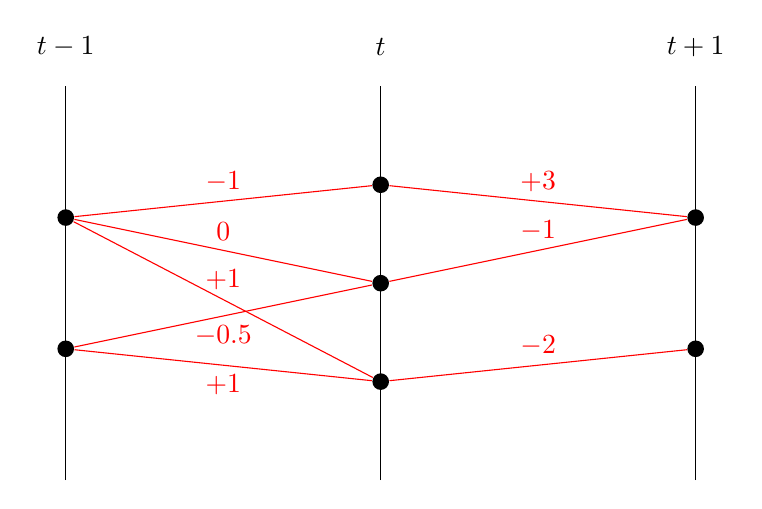
\begin{tikzpicture}
      \draw (0,0) -- (0,5);%
      \draw (4,0) -- (4,5);%
      \draw (8,0) -- (8,5);%

      \node[circle,inner sep=0pt, minimum size=6pt,fill] (A1) at (0,1.6666) {};%
      \node[circle,inner sep=0pt, minimum size=6pt,fill] (A2) at (0,3.3333) {};%

      \node[circle,inner sep=0pt, minimum size=6pt,fill] (B1) at (4,1.25) {};%
      \node[circle,inner sep=0pt, minimum size=6pt,fill] (B2) at (4,2.5) {};%
      \node[circle,inner sep=0pt, minimum size=6pt,fill] (B3) at (4,3.75) {};%

      \node[circle,inner sep=0pt, minimum size=6pt,fill] (C1) at (8,1.6666) {};%
      \node[circle,inner sep=0pt, minimum size=6pt,fill] (C2) at (8,3.3333) {};%

      \draw[red] (A1) -- (B1) node[midway,below] {$+1$};%
      \draw[red] (A1) -- (B2) node[midway,below] {$-0.5$};%
      \draw[red] (A2) -- (B1) node[midway,above] {$+1$};%
      \draw[red] (A2) -- (B2) node[midway,above] {$0$};%
      \draw[red] (A2) -- (B3) node[midway,above] {$-1$};%

      \draw[red] (B1) -- (C1) node[midway,above] {$-2$};%
      \draw[red] (B2) -- (C2) node[midway,above] {$-1$};%
      \draw[red] (B3) -- (C2) node[midway,above] {$+3$};%

      \node at (0,5.5) {$t-1$};%
      \node at (4,5.5) {$t$};%
      \node at (8,5.5) {$t+1$};%
    \end{tikzpicture}
    \caption{Detections (black dots) at three time steps with assignments and
      costs.}
  \end{subfigure}
  \begin{subfigure}{\textwidth}
    \centering
    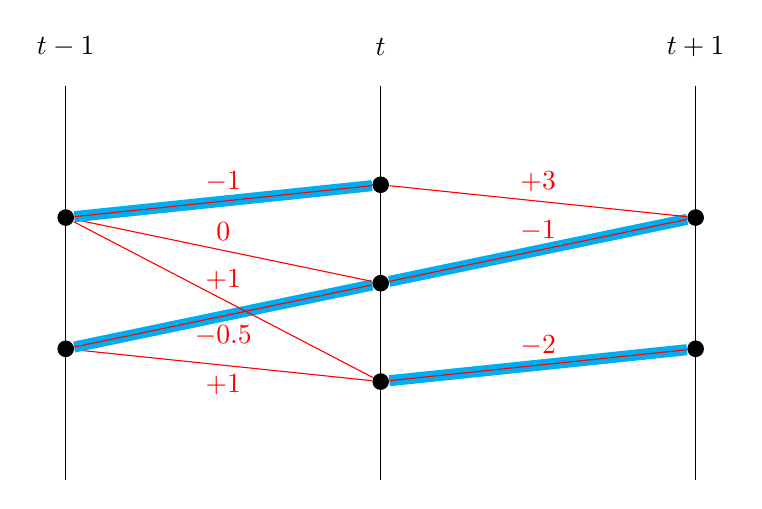
\begin{tikzpicture}
      \draw (0,0) -- (0,5);%
      \draw (4,0) -- (4,5);%
      \draw (8,0) -- (8,5);%

      \node[circle,inner sep=0pt, minimum size=6pt,fill] (A1) at (0,1.6666) {};%
      \node[circle,inner sep=0pt, minimum size=6pt,fill] (A2) at (0,3.3333) {};%

      \node[circle,inner sep=0pt, minimum size=6pt,fill] (B1) at (4,1.25) {};%
      \node[circle,inner sep=0pt, minimum size=6pt,fill] (B2) at (4,2.5) {};%
      \node[circle,inner sep=0pt, minimum size=6pt,fill] (B3) at (4,3.75) {};%

      \node[circle,inner sep=0pt, minimum size=6pt,fill] (C1) at (8,1.6666) {};%
      \node[circle,inner sep=0pt, minimum size=6pt,fill] (C2) at (8,3.3333) {};%

      \draw[red] (A1) -- (B1) node[midway,below] {$+1$};%
      \draw[red,preaction={ draw,cyan,-,double=cyan, double
        distance=8\pgflinewidth, }] (A1) -- (B2) node[midway,below] {$-0.5$};%
      \draw[red] (A2) -- (B1) node[midway,above] {$+1$};%
      \draw[red] (A2) -- (B2) node[midway,above] {$0$};%
      \draw[red,preaction={ draw,cyan,-,double=cyan, double
        distance=8\pgflinewidth, }] (A2) -- (B3) node[midway,above] {$-1$};%

      \draw[red,preaction={ draw,cyan,-,double=cyan, double
        distance=8\pgflinewidth, }] (B1) -- (C1) node[midway,above] {$-2$};%
      \draw[red,preaction={ draw,cyan,-,double=cyan, double
        distance=8\pgflinewidth, }] (B2) -- (C2) node[midway,above] {$-1$};%
      \draw[red] (B3) -- (C2) node[midway,above] {$+3$};%

      \node at (0,5.5) {$t-1$};%
      \node at (4,5.5) {$t$};%
      \node at (8,5.5) {$t+1$};%
    \end{tikzpicture}
    \caption{Matching detections only in pairs of frames. The results are not
      consistent across frames.}
  \end{subfigure}
  \begin{subfigure}{\textwidth}
    \centering
    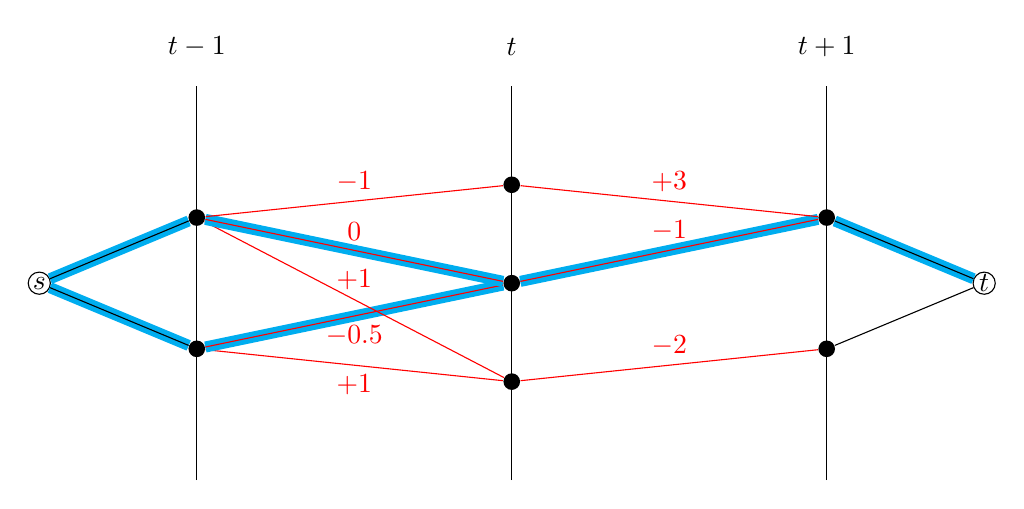
\begin{tikzpicture}
      \draw (0,0) -- (0,5);%
      \draw (4,0) -- (4,5);%
      \draw (8,0) -- (8,5);%

      \node[circle,inner sep=0pt, minimum size=6pt,fill] (A1) at (0,1.6666) {};%
      \node[circle,inner sep=0pt, minimum size=6pt,fill] (A2) at (0,3.3333) {};%

      \node[circle,inner sep=0pt, minimum size=6pt,fill] (B1) at (4,1.25) {};%
      \node[circle,inner sep=0pt, minimum size=6pt,fill] (B2) at (4,2.5) {};%
      \node[circle,inner sep=0pt, minimum size=6pt,fill] (B3) at (4,3.75) {};%

      \node[circle,inner sep=0pt, minimum size=6pt,fill] (C1) at (8,1.6666) {};%
      \node[circle,inner sep=0pt, minimum size=6pt,fill] (C2) at (8,3.3333) {};%

      \node[draw,circle,inner sep=0pt, minimum size=8pt] (S) at (-2,2.5) {$s$};%
      \node[draw,circle,inner sep=0pt, minimum size=8pt] (T) at (10,2.5) {$t$};%
      
      \draw[red] (A1) -- (B1) node[midway,below] {$+1$};%
      \draw[red,preaction={ draw,cyan,-,double=cyan, double
        distance=8\pgflinewidth, }] (A1) -- (B2) node[midway,below] {$-0.5$};%
      \draw[red] (A2) -- (B1) node[midway,above] {$+1$};%
      \draw[red,preaction={ draw,cyan,-,double=cyan, double
        distance=8\pgflinewidth, }] (A2) -- (B2) node[midway,above] {$0$};%
      \draw[red] (A2) -- (B3) node[midway,above] {$-1$};%

      \draw[red] (B1) -- (C1) node[midway,above] {$-2$};%
      \draw[red,preaction={ draw,cyan,-,double=cyan, double
        distance=8\pgflinewidth, }] (B2) -- (C2) node[midway,above] {$-1$};%
      \draw[red] (B3) -- (C2) node[midway,above] {$+3$};%

      \draw[black,preaction={ draw,cyan,-,double=cyan, double
        distance=8\pgflinewidth, }] (S) -- (A2);%
      \draw[black,preaction={ draw,cyan,-,double=cyan, double
        distance=8\pgflinewidth, }] (S) -- (A1);%

      \draw[black] (C1) -- (T);%
      \draw[black,preaction={ draw,cyan,-,double=cyan, double
        distance=8\pgflinewidth, }] (C2) -- (T);%
      
      \node at (0,5.5) {$t-1$};%
      \node at (4,5.5) {$t$};%
      \node at (8,5.5) {$t+1$};%
    \end{tikzpicture}
    \caption{Matching detections using the shortest path and second shortest
      path. A single edge is used more than once which is not desired.}
  \end{subfigure}
  \caption{Example for tracking without division.}%
  \label{fig:tracking}
\end{figure}

Hence, we need another way to find suitable paths in this graph to which end we
introduce the notion of min-cost flows. In this setting we again assume that
paths are additive along paths. The min-cost flow formulation of the problem
enforces the laws of conservation and we can impose a restriction on the number
of times one vertex can be used, which in our case would be one. To demonstrate
the idea, we have to slightly modify the graph from above, the results is shown
in Figure~\ref{fig:min-cost}. There, we have duplicated each ``layer'' of the
graph and connected the two arsing layers to each other (the blue edges). The
purpose of this modification is as follows. Sometimes we might assign a cost (or
a reward) to certain implausible (or very plausible) detections. This can now be
achieved by assigning a cost (reward) of accepting to the blue edges which. This
formulation also allows to easily model spontaneous appearing and disappearing
detections. To model appearing detections we can add edges from the starting
node to any of the edges in the first parts of the second or third layer and
analogously, we can add edges from the second parts of the layers to the target
vertex to model spontaneous disappearance. In the figure we also indicated the
optimal min-cost flow solution; before discussing how to obtain these solutions
in the general case, we first define the precise optimisation problem that we
try to solve.

\begin{figure}[htpb]
  \centering
  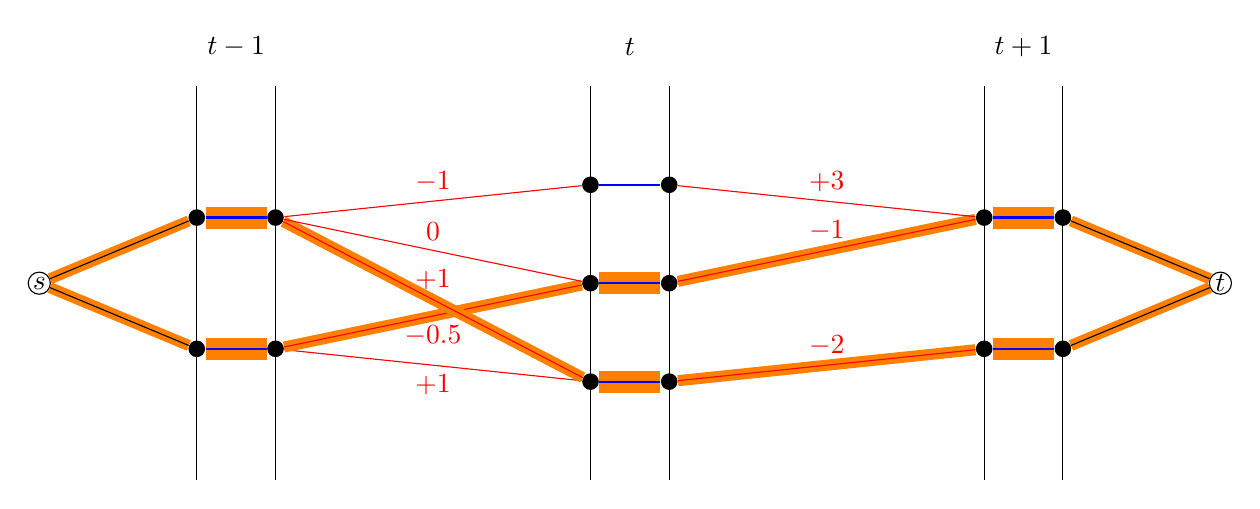
\begin{tikzpicture}
    \draw (0,0) -- (0,5);%
    \draw (1,0) -- (1,5);%
    \draw (5,0) -- (5,5);%
    \draw (6,0) -- (6,5);%
    \draw (10,0) -- (10,5);%
    \draw (11,0) -- (11,5);%

    \node[circle,inner sep=0pt, minimum size=6pt,fill] (A1) at (0,1.6666) {};%
    \node[circle,inner sep=0pt, minimum size=6pt,fill] (A2) at (0,3.3333) {};%
    \node[circle,inner sep=0pt, minimum size=6pt,fill] (A3) at (1,1.6666) {};%
    \node[circle,inner sep=0pt, minimum size=6pt,fill] (A4) at (1,3.3333) {};%
    

    \node[circle,inner sep=0pt, minimum size=6pt,fill] (B1) at (5,1.25) {};%
    \node[circle,inner sep=0pt, minimum size=6pt,fill] (B2) at (5,2.5) {};%
    \node[circle,inner sep=0pt, minimum size=6pt,fill] (B3) at (5,3.75) {};%
    \node[circle,inner sep=0pt, minimum size=6pt,fill] (B4) at (6,1.25) {};%
    \node[circle,inner sep=0pt, minimum size=6pt,fill] (B5) at (6,2.5) {};%
    \node[circle,inner sep=0pt, minimum size=6pt,fill] (B6) at (6,3.75) {};%

    \node[circle,inner sep=0pt, minimum size=6pt,fill] (C1) at (10,1.6666) {};%
    \node[circle,inner sep=0pt, minimum size=6pt,fill] (C2) at (10,3.3333) {};%
    \node[circle,inner sep=0pt, minimum size=6pt,fill] (C3) at (11,1.6666) {};%
    \node[circle,inner sep=0pt, minimum size=6pt,fill] (C4) at (11,3.3333) {};%

    \node[draw,circle,inner sep=0pt, minimum size=8pt] (S) at (-2,2.5) {$s$};%
    \node[draw,circle,inner sep=0pt, minimum size=8pt] (T) at (13,2.5) {$t$};%
      
    \draw[red] (A3) -- (B1) node[midway,below] {$+1$};%
    \draw[red,preaction={ draw,orange,-,double=orange, double
      distance=8\pgflinewidth, }] (A3) -- (B2) node[midway,below] {$-0.5$};%
    \draw[red,preaction={ draw,orange,-,double=orange, double
      distance=8\pgflinewidth, }] (A4) -- (B1) node[midway,above] {$+1$};%
    \draw[red] (A4) -- (B2) node[midway,above] {$0$};%
    \draw[red] (A4) -- (B3) node[midway,above] {$-1$};%

    \draw[red,preaction={ draw,orange,-,double=orange, double
      distance=8\pgflinewidth, }] (B4) -- (C1) node[midway,above] {$-2$};%
    \draw[red,preaction={ draw,orange,-,double=orange, double
      distance=8\pgflinewidth, }] (B5) -- (C2) node[midway,above] {$-1$};%
    \draw[red] (B6) -- (C2) node[midway,above] {$+3$};%

    \draw[black,preaction={ draw,orange,-,double=orange, double
      distance=8\pgflinewidth, }] (S) -- (A2);%
    \draw[black,preaction={ draw,orange,-,double=orange, double
      distance=8\pgflinewidth, }] (S) -- (A1);%

    \draw[black,preaction={ draw,orange,-,double=orange, double
      distance=8\pgflinewidth, }] (C3) -- (T);%
    \draw[black,preaction={ draw,orange,-,double=orange, double
      distance=8\pgflinewidth, }] (C4) -- (T);%

    \draw[blue,thick,preaction={ draw,orange,-,double=orange, double
      distance=8\pgflinewidth, }] (A1) -- (A3);%
    \draw[blue,thick,preaction={ draw,orange,-,double=orange, double
      distance=8\pgflinewidth, }] (A2) -- (A4);%

    \draw[blue,thick,preaction={ draw,orange,-,double=orange, double
      distance=8\pgflinewidth, }] (B1) -- (B4);%
    \draw[blue,thick,preaction={ draw,orange,-,double=orange, double
      distance=8\pgflinewidth, }] (B2) -- (B5);%
    \draw[blue,thick] (B3) -- (B6);%

    \draw[blue,thick,preaction={ draw,orange,-,double=orange, double
      distance=8\pgflinewidth, }] (C1) -- (C3);%
    \draw[blue,thick,preaction={ draw,orange,-,double=orange, double
      distance=8\pgflinewidth, }] (C2) -- (C4);%
      
    \node at (0.5,5.5) {$t-1$};%
    \node at (5.5,5.5) {$t$};%
    \node at (10.5,5.5) {$t+1$};%
  \end{tikzpicture}
  \caption{Min-cost flow formulation of the previous problem.}%
  \label{fig:min-cost}
\end{figure}

To that end, we consider a graph $G(V,E)$ with vertices $V$ and edges $E$ in
which we want to find a flow $x$ (note, that the graphs in the examples are
actually directed; we omitted the arrows that would indicate the directions
since in our case the direction is always from left to right). The optimisation
problem can now be written as
\begin{equation*}
  \text{Find }\ \min_x \sum_{e \in E}x_e c_e\,,
\end{equation*}
where $x_e$ is the flow across edge $e$ and $c_e$ is the cost of sending one
unit of flow across edge $e$. That is, $c_e$ is the cost of using an edge while
$x_e$ is the number of times an edge is used. To ensure that flows go from the
starting node to the target node, we impose the following conservation law for
all $v \in V \setminus \{s,t\}$
\begin{equation*}
  \sum_{u:\,(u,v)\in E} x_{(u,v)} =  \sum_{w:\,(v,w)\in E} x_{(v,w)}\,.
\end{equation*}
This ensures that all for every oncoming connection to a node $v$, there is also
an outgoing connection from $v$. To ensure that the flow should not exceed a
certain upper limit, \ie a certain capacity on a particular edge, we add the
following constraint for all edges $e$
\begin{equation*}
  x_e \le b_e\,,
\end{equation*}
where $b_e$ is the bottleneck associated with the edge $e$. In our example
above, we would have $b_e \le 1$. In many tracking problems, we can also impose
an integral constraint such as
\begin{equation*}
  x_e \in \{0,1\}\,.
\end{equation*}
This ensures that there cannot be half a person, or half a cell that is tracked
but that one detections corresponds to one instance. Note that this last
assumptions makes the problem non-convex and thus hard to solve but luckily,
this constraint can be replaced by the convex constraint $x_e \ge 0$ for
min-cost flow problems.

\subsection*{Linear Programming}
We can rewrite the problem above in the canonical form of an eminent
optimisation problem, a so called \emph{Integer Linear Program} or ILP, for
short. We start by defining what we mean by a linear program. It is the
following optimisation problem
\begin{equation*}
  \min_x c^\tp x \qquad \text{s.t.}\quad Ax \le b \quad \text{and}\quad x\ge 0\,.
\end{equation*}
This is a convex problem and is thus easy to solve (using the Simplex algorithm
or the interior point method). If we add the following integer restriction
\begin{equation*}
  x \in \Z^{\dim(x)}\,,
\end{equation*}
the problem becomes non-convex and solving it is now NP-hard.

\todo{Add feasible region figure}

In summary, we have seen that we can model tracking-by-assignment as a
minimum-cost flow problem and thus as a linear program which can be solved to
global optimality efficiently (in polynomial time). Integer linear programs, on
the other hand, are usually very hard to solve; however, if the have certain
special structures they can sometimes be reduced to easier problems. For
instance, if the constraint matrix is totally unimodular and the right hand side
is integer-valued, the problem can be reduced to a standard linear
program. Also, shortest path problems (or more generally, flow problems) are
only one instance of ILPs that happen to be easy to solve.

\section{Total Unimodularity}
As mentioned above, under certain circumstances can an ILP be solved
efficiently, for instance when the constraint matrix is totally unimodular.
\begin{definition}
  Let $A \in \Z^{m \times n}$ be an integer matrix.
  \begin{enumerate}[label=(\alph*)]
  \item If $A$ is square, we say $A$ is \emph{unimodular} if $\det(A) = \pm 1$.
  \item $A$ is called \emph{totally unimodular} if for every submatrix $B$ of
    $A$ it holds that $\det(B) \in \{-1,0,1\}$.
  \end{enumerate}
  One can show that every for entry $a_{ij}$ of totally unimodular matrix $A$ it
  holds that $a_{ij} \in \{-1,0,1\}$, which is not true for unimodular matrices.
\end{definition}

As mentioned above, if the constraint matrix of a ILP is totally unimodular and
the right hand side is integer-valued, the ILP can be solved efficiently. This
is due to the fact that in this case the feasible region has integer vertices
only which implies that the integer linear program solution coincides with the
normal linear program solution. It turns out that any min-cost flow problem with
integer edge capacities that does not have negative cost cycles has an optimal
solution with integer flows on its edges.

A main ingredient of proofing the results above is the following fact. The
linear equation $Bx = b$ with a non-singular integer-valued square matrix $B$
and an integer-valued vector $b$ has an integer-valued solution $x$ if and only
if $B$ is unimodular.

In summary, ``pure'' flow problems (max-/min-cost flow problems) can be
described by linear programs with totally unimodular constraint matrices.  Given
integer edge flow bounds (right hand sides in the LP), this guarantees integral
solutions of the optimisation problem. Hence, such pure flow problems can be
efficiently solved to global optimality.

%%% Local Variables:
%%% mode: latex
%%% TeX-master: "../main"
%%% End:
